
\documentclass[a4paper,11pt]{article}

% -------------------------------------------------
% ENCODING / LANGUAGE
% -------------------------------------------------
\usepackage[utf8]{inputenc}
\usepackage[T1]{fontenc}
\usepackage[english]{babel}

% -------------------------------------------------
% MATH / SCIENCE
% -------------------------------------------------
\usepackage{amsmath,amssymb,amsfonts}
\usepackage{array}
\usepackage{booktabs}
\usepackage{multirow}
\usepackage{tabularx}
\usepackage{longtable}

% -------------------------------------------------
% LAYOUT / STYLE
% -------------------------------------------------
\usepackage[top=2.5cm,bottom=2.5cm,left=2.25cm,right=2.25cm]{geometry}
\usepackage{setspace}
\usepackage{indentfirst}
\usepackage{fancyhdr}
\usepackage{xcolor}
\usepackage{graphicx}
\usepackage{tikz}
\usepackage{hyperref}
\usepackage{enumitem}
\usepackage{titlesec}
\usepackage{tocloft}
\usepackage{caption}
\usepackage{listings}
\usepackage[numbers]{natbib}
\usepackage{float}

\onehalfspacing
\setlength{\parskip}{0.2em}
\setlength{\parindent}{15pt}

% -------------------------------------------------
% HYPERREF
% -------------------------------------------------
\hypersetup{
  colorlinks=true,
  linkcolor=black,
  citecolor=black,
  urlcolor=blue,
  pdftitle={Self-Supervised Test-Time Training for Image Classification},
  pdfauthor={Rayane KHATIM, Mehdi AGHAEI},
  pdfsubject={Research project},
  pdfkeywords={test-time training, SimCLR, CIFAR-10-C, ActMAD}
}

% -------------------------------------------------
% CODE LISTINGS
% -------------------------------------------------
\lstset{
  basicstyle=\ttfamily\footnotesize,
  backgroundcolor=\color{gray!10},
  frame=single,
  breaklines=true,
  showstringspaces=false,
  numbers=none
}

% -------------------------------------------------
% HEADER / FOOTER
% -------------------------------------------------
\pagestyle{fancy}
\fancyhf{}
\fancyhead[L]{Paris Cite University}
\fancyhead[R]{Rayane KHATIM - Mehdi AGHAEI}
\fancyfoot[L]{Research Project}
\fancyfoot[R]{\thepage}
\renewcommand{\headrulewidth}{0.4pt}
\renewcommand{\footrulewidth}{0.4pt}
\setlength{\headheight}{14pt}

% -------------------------------------------------
% SECTION STYLE
% -------------------------------------------------
\titleformat{\section}{\large\bfseries}{\thesection}{1em}{}
\titleformat{\subsection}{\normalsize\bfseries}{\thesubsection}{1em}{}
\titleformat{\subsubsection}{\normalsize\itshape}{\thesubsubsection}{1em}{}

% -------------------------------------------------
% COMPACT TABLE OF CONTENTS
% -------------------------------------------------
\setlength{\cftbeforetoctitleskip}{0pt}
\setlength{\cftaftertoctitleskip}{0.35em}
\setlength{\cftbeforesecskip}{0.12em}
\setlength{\cftbeforesubsecskip}{0pt}
\renewcommand{\cfttoctitlefont}{\large\bfseries}
\renewcommand{\cftsecfont}{\small\bfseries}
\renewcommand{\cftsecpagefont}{\small\bfseries}
\renewcommand{\cftsubsecfont}{\small}
\renewcommand{\cftsubsecpagefont}{\small}

% -------------------------------------------------
% CUSTOM COMMANDS
% -------------------------------------------------
\newcommand{\MainTitle}{RESEARCH PROJECT}
\newcommand{\ProjectTitle}{Self-Supervised Test-Time Training for Image Classification}
\newcommand{\ReportDate}{MAY 2026}
\newcommand{\InstitutionName}{PARIS CITE UNIVERSITY}
\newcommand{\missing}{\textit{Not provided in the available results.}}
\newcommand{\pp}{percentage points}
\graphicspath{{figures/}}

\begin{document}
\sloppy

% =================================================
% COVER PAGE
% =================================================
\begin{titlepage}
\thispagestyle{empty}

\begin{center}
{\Large \InstitutionName \par}
\end{center}

\vspace{2.0cm}

\begin{center}
{\fontsize{20}{25}\selectfont \bfseries \MainTitle \par}
\vspace{0.6cm}
{\fontsize{15}{20}\selectfont \bfseries \ProjectTitle \par}
\vspace{1.2cm}
{\Large \ReportDate \par}
\end{center}

\vspace{1.8cm}

\begin{center}
\textbf{Authors:}\\[0.35cm]
\begin{tabular}{cc}
Rayane KHATIM & Mehdi AGHAEI\\
\texttt{rayane.khatim@etu.u-paris.fr} & \texttt{mehdi.aghaei@etu.u-paris.fr}\\
22500285 & 22500371
\end{tabular}
\end{center}

\vspace{1.2cm}

\begin{center}
\textbf{Supervisors:}\\[0.25cm]
Prof. Ayoub Karine : \texttt{ayoub.karine@u-paris.fr}\\
Prof. Camille Kurtz : \texttt{camille.kurtz@u-paris.fr}\\
Prof. Laurent Wendling : \texttt{Laurent.Wendling@u-paris.fr}
\end{center}

\vfill

\begin{center}
\rule{0.75\textwidth}{0.4pt}
\end{center}

\end{titlepage}

\tableofcontents
\newpage

% =================================================
\section{Introduction and Context}
% =================================================

Image classification models usually work well when the test images are close to the images used during training. This assumption is weak in practice. A camera image can contain sensor noise, blur, compression artifacts, fog, snow, low contrast, or a strong change in brightness. These changes do not necessarily change the object class, but they change the input distribution seen by the model. A network trained only on clean images can then make unstable predictions, even when the image is still understandable for a human observer.

This project studies that problem in a controlled computer vision setting. CIFAR-10 is used as the clean source domain \citep{krizhevsky2009cifar}. The target domain is based on corrupted CIFAR-10 images, following the CIFAR-10-C evaluation idea \citep{hendrycks2019robustness}. CIFAR-10-C is useful because it separates common corruptions into named corruption types and severity levels. It is not an adversarial benchmark. The corruptions are ordinary image degradations: noise, blur, weather effects, digital compression, contrast changes, and geometric distortions.

The project does not try to design a new backbone architecture. The backbone is ResNet18 \citep{he2016resnet}, and the representation is trained with SimCLR, a self-supervised contrastive method \citep{chen2020simclr}. The main question is narrower: after the model has been trained on source data, can it adapt itself at test time using only an unlabeled corrupted batch? If this adaptation improves accuracy, the model becomes less dependent on perfectly clean test data. If it decreases accuracy, the adaptation objective is not aligned well enough with classification.

The adaptation strategy implemented in the project is ActMAD-style activation matching \citep{mirza2023actmad}. The model first records activation statistics on clean source data. At test time, it receives a corrupted batch and updates a limited subset of parameters so that the target activations become closer to the source activations. The current implementation adapts normalization parameters and keeps the rest of the model frozen. The classification head is then applied after this short adaptation.

The final available run gives a useful but limited result. SimCLR training completed for 100 epochs, and the linear evaluation accuracy reached 67.05\%. The available test-time evaluation improved from 48.34\% without adaptation to 55.78\% after ActMAD TTT. The gain is 7.44 percentage points. At the same time, an attempted official CIFAR-10-C run failed because \texttt{data/raw/cifar10c/CIFAR-10-C/shot\_noise.npy} was missing. The report therefore treats the available TTT result as a confirmed evaluation output, not as a complete official CIFAR-10-C benchmark.

% =================================================
\section{Scientific Background and Related Work}
% =================================================

\subsection{Supervised image classification and distribution shift}

In supervised image classification, the model learns a function
\[
f_\theta : \mathcal{X} \rightarrow \{1,\ldots,K\}
\]
from images to class labels. For CIFAR-10, \(K=10\). The usual training objective assumes that the training and test examples are sampled from similar distributions. Under that condition, minimizing the training loss can lead to good test accuracy if the model generalizes correctly.

The problem changes when the test distribution is shifted. A corrupted image may still contain the same semantic object, but the low-level statistics can be different. Noise modifies pixel values. Blur removes high-frequency details. Compression creates blocks and artifacts. Fog and brightness changes affect contrast and color distributions. Since convolutional neural networks learn a mixture of low-level and high-level features, these changes can propagate through the network and modify the internal activations.

CIFAR-10-C was introduced as part of the common corruptions benchmark proposed by Hendrycks and Dietterich \citep{hendrycks2019robustness}. The benchmark is useful because it avoids vague robustness claims. A method can be tested on fixed corruptions and severity levels. If the full benchmark is used, accuracy or error can be reported per corruption and then averaged. In this project, the official CIFAR-10-C format is treated as the correct final benchmark. The provided final log does not prove a full official CIFAR-10-C evaluation, so the report does not claim one.

\subsection{Self-supervised representation learning}

Self-supervised learning uses labels created from the data itself. The goal is not to predict the final class label directly, but to learn a representation that contains useful structure. After pretraining, a smaller supervised head can be trained on top of the frozen representation. This is often called linear evaluation when the head is a linear classifier.

SimCLR is a contrastive self-supervised method \citep{chen2020simclr}. For each image, two different augmented views are generated. The model should map these two views close to each other in representation space. Views from different images should be separated. This gives a training signal without class labels. For this project, SimCLR is a good fit because CIFAR-10 can provide many augmented image pairs, and the learned backbone can later be reused for classification and test-time adaptation.

The implementation uses a ResNet18 backbone and a projection head. The backbone produces a feature vector. The projection head maps this feature vector into the contrastive space used for the SimCLR loss. The classifier is not trained during contrastive pretraining. It is trained later during linear evaluation on frozen features.

\subsection{Contrastive learning and NT-Xent loss}

Let \(x_i\) be an image and let \(t_1\) and \(t_2\) be two stochastic augmentations. SimCLR builds two views:
\[
\tilde{x}_{i,1}=t_1(x_i),\qquad \tilde{x}_{i,2}=t_2(x_i).
\]
The encoder and projection head map them to normalized vectors \(z_{i,1}\) and \(z_{i,2}\). These two vectors are a positive pair. The other views in the same batch act as negative examples.

The project uses the NT-Xent loss. For a positive pair \((i,j)\), a simplified form is:
\[
\ell_{i,j}=-\log \frac{\exp(\operatorname{sim}(z_i,z_j)/\tau)}{\sum_{k\neq i}\exp(\operatorname{sim}(z_i,z_k)/\tau)},
\]
where \(\operatorname{sim}\) is a similarity score and \(\tau\) is the temperature. In the code, the projected vectors are normalized and the similarity matrix is computed by a dot product. The diagonal is masked because each view should not be compared with itself. The target label for each view is the index of its paired augmented view.

This loss is not a classification loss. It does not know the CIFAR-10 class names. It only asks the network to learn invariances induced by the augmentation pipeline. If the augmentations are well chosen, the representation captures useful image structure. If the augmentations are too weak or too strong, the representation can become less useful for classification.

\subsection{Linear evaluation}

Linear evaluation is a practical check of representation quality. After SimCLR pretraining, the backbone is frozen. A linear classifier is trained on top of the features using class labels. A high linear evaluation accuracy means that the frozen representation already separates classes well enough for a simple head. A low linear evaluation accuracy means that the representation is weak or not aligned with the classification task.

This matters for TTT. Test-time adaptation cannot fully repair a poor representation. If the backbone does not extract useful features before adaptation, then matching activation statistics may not be enough. The final run reached 67.05\% linear evaluation accuracy. This is much stronger than the earlier one-epoch smoke result, but it is still limited compared with a strong fully supervised CIFAR-10 classifier. The number is therefore useful evidence of learned features, not evidence that the backbone is optimal.

\subsection{Test-Time Training and test-time adaptation}

Test-Time Training adapts a model during inference using an auxiliary objective that does not need labels \citep{sun2020ttt}. A model trained on a source domain receives target-domain inputs at test time. Before predicting labels, it performs a few gradient steps on a self-supervised or unsupervised loss. The goal is to move the model toward the target distribution without using target labels.

The difficulty is that the auxiliary loss is not the classification loss. It may improve the internal representation, but it may also move the model in a harmful direction. TTT++ studies this instability and shows that self-supervised test-time training can fail under some shifts \citep{liu2021tttpp}. A positive result on one evaluated setting is useful, but it does not prove that the method is safe for all corruptions.

Test-time adaptation is attractive because it does not require labeled target data. In many applications, labeled target data is not available when the distribution changes. The model only sees new unlabeled images. This matches the project setting: target batches from corrupted CIFAR-10 images are available, but their labels should not be used for adaptation.

\subsection{ActMAD and activation matching}

ActMAD proposes to adapt a model by matching activation distributions between source data and test-time data \citep{mirza2023actmad}. The intuition is that a distribution shift changes internal activations. If the model can adjust itself so that target activations become closer to source activations, its predictions may become more stable.

The project implements a simplified ActMAD-style objective. During a source-statistics phase, hooks record the activations of normalization layers on clean data. For each layer, the code computes a mean and a standard deviation. During adaptation, the target batch is passed through the model, target activation statistics are computed, and the loss penalizes the difference between target and source statistics. In simplified notation, for layers \(l\in\mathcal{L}\):
\[
\mathcal{L}_{\text{ActMAD}}=\frac{1}{|\mathcal{L}|}\sum_{l\in\mathcal{L}}\left(\|\mu_l^t-\mu_l^s\|_2^2+\|\sigma_l^t-\sigma_l^s\|_2^2\right).
\]
Here, \(\mu_l^s\) and \(\sigma_l^s\) are source statistics. The target statistics \(\mu_l^t\) and \(\sigma_l^t\) are computed on the current unlabeled target batch. This loss does not use image labels.

% =================================================
\section{Problem Formulation}
% =================================================

The source domain is the clean CIFAR-10 distribution. It contains image-label pairs \((x_s,y_s)\) sampled from \(D_s\). The target domain contains corrupted CIFAR-10 images sampled from \(D_t\). The labels still correspond to the same ten CIFAR-10 classes, but they are not used during adaptation.

The baseline prediction is obtained by applying the trained backbone and classifier directly to the corrupted batch:
\[
\hat{y}_{\text{base}}=\arg\max f_\theta(x_t).
\]
The adapted prediction first creates a temporary adapted model. A few gradient steps are applied on the unlabeled target batch using the activation matching loss. The prediction is then computed with the adapted parameters:
\[
\hat{y}_{\text{ttt}}=\arg\max f_{\theta'}(x_t),\qquad \theta'=\theta-\alpha\nabla_\theta\mathcal{L}_{\text{ActMAD}}(x_t).
\]
In the current implementation, not all parameters are adapted. Most of the model is frozen, and only normalization layer parameters are updated.

The evaluation compares top-1 accuracy before and after adaptation. The improvement is reported in percentage points:
\[
\Delta=\operatorname{Acc}_{\text{TTT}}-\operatorname{Acc}_{\text{base}}.
\]
A positive value means the adaptation improved accuracy. A negative value means the adaptation damaged accuracy. This sign is important because test-time adaptation should not be described as successful if it improves one setting and fails on another.

The report separates three cases. The first is clean CIFAR-10 source training and linear evaluation. The second is official CIFAR-10-C evaluation, which requires the official \texttt{.npy} corruption files. The third is an available local TTT evaluation. The final terminal output confirms the first and the third. It also confirms that one attempted official CIFAR-10-C run failed because \texttt{shot\_noise.npy} was missing.

% =================================================
\section{Methodology}
% =================================================

\subsection{SimCLR pretraining on CIFAR-10}

The first stage trains a self-supervised encoder on CIFAR-10. The loader returns two augmented views of each image. The augmentations used in the repository include random resized cropping, horizontal flipping, color jitter, random grayscale conversion, conversion to tensor, and CIFAR-10 normalization. These transformations are defined in \texttt{src/datasets.py} through the two-view transformation used for SimCLR.

The model is defined in \texttt{src/self\_supervised.py}. It uses a torchvision ResNet18 with the final classification layer replaced by an identity mapping. The output of the backbone is then passed through a projection head. The projection head is a small multilayer perceptron with a linear layer, ReLU activation, and another linear layer. The output is normalized before the contrastive loss.

For each batch, the training loop computes two projected representations, one for each view. The NT-Xent loss is then applied. The optimizer used in the current code is Adam. A cosine annealing scheduler is also created. The final run completed all 100 epochs and printed the training loss at each epoch.

\subsection{Feature extraction and projection head}

The backbone and projection head serve different roles. The projection head is useful for contrastive pretraining, but the classifier is trained on the raw backbone features. This is standard in SimCLR-style evaluation: the projection space helps the contrastive loss, while the representation before projection is used for downstream tasks.

In the code, the SimCLR forward path returns projected features for the SSL loss. The encoding path returns the raw backbone features. Linear evaluation uses the encoded backbone features, not the projection output. This distinction avoids forcing the final classifier to operate in the contrastive projection space.

\subsection{Linear classifier on frozen features}

After pretraining, the backbone parameters are frozen. The linear evaluation step trains a linear layer with ten output classes. In the inspected implementation, this classifier is trained with Adam. The classifier is saved as:
\begin{lstlisting}
results/self_supervised/classifier.pt
\end{lstlisting}
The backbone checkpoint used for TTT is saved as:
\begin{lstlisting}
results/self_supervised/simclr_backbone.pt
\end{lstlisting}

Linear evaluation is not the final project goal, but it gives an important diagnostic. The final value is 67.05\%. This means the self-supervised representation contains useful class information. It also shows that the representation is not extremely strong. The later TTT result should be read with that limitation in mind.

\subsection{Source activation statistics}

Before test-time adaptation, the project computes source activation statistics. The code registers forward hooks on BatchNorm and LayerNorm modules. For each selected layer, it records activations on clean source validation data and computes mean and standard deviation across the appropriate dimensions.

The result is saved as:
\begin{lstlisting}
results/self_supervised/source_stats.pt
\end{lstlisting}
This file is required by the TTT stage. It represents the clean source-domain activation reference. During adaptation, the corrupted target batch is pushed toward these reference statistics.

\subsection{ActMAD-style adaptation at test time}

The TTT stage is implemented in \texttt{src/test\_time\_training.py}. The adapter stores the base model and source statistics. For each target batch, the adapter creates a deep copy of the base model. This is important because test-time updates should not permanently modify the original model across unrelated batches. Without a fresh copy, adaptation errors could accumulate from batch to batch.

The copied model is put in training mode. All parameters are frozen first. Then, only parameters inside normalization modules are made trainable. The adaptation optimizer is Adam. The public TTT configuration uses ActMAD, ten adaptation steps per batch, learning rate \(10^{-4}\), and the source statistics stored in \texttt{results/self\_supervised/source\_stats.pt}.

At each adaptation step, the model processes the unlabeled target batch, the activation matching loss is computed, and the normalization parameters are updated. After the adaptation steps, the copied model is used for prediction. This design is cautious. It does not fine-tune the full network at test time. Updating all weights on a small unlabeled batch would be risky and expensive. Updating only normalization parameters is more limited, but it is less likely to destroy the learned representation.

% =================================================
\section{Implementation Details}
% =================================================

\subsection{Repository structure}

The project repository is organized around one entry point and several modules. The main command-line file is \texttt{run.py}. It accepts two main tasks:
\begin{itemize}[leftmargin=1.4em]
\item \texttt{self\_supervised}, also available as \texttt{ssl};
\item \texttt{test\_time\_training}, also available as \texttt{ttt}.
\end{itemize}

The GitHub README describes the repository as a Master 1 TER project focused on Test-Time Training and Self-Supervised Learning, with authors Rayane KHATIM and Mehdi AGHAEI. The main folders are \texttt{configs/}, \texttt{src/}, \texttt{scripts/}, \texttt{data/}, \texttt{papers/}, \texttt{docs/}, \texttt{notebooks/}, \texttt{presentation/}, and \texttt{report/}.

The implementation files used by the report are:
\begin{itemize}[leftmargin=1.4em]
\item \texttt{run.py}: argument parsing, task selection, checkpoint loading, and high-level execution;
\item \texttt{src/self\_supervised.py}: SimCLR model, projection head, NT-Xent loss, SSL trainer, linear evaluation, and source-statistics call;
\item \texttt{src/test\_time\_training.py}: activation hooks, source statistics, ActMAD loss, and TTT adapter;
\item \texttt{src/datasets.py}: CIFAR-10 loaders, SimCLR two-view transform, and CIFAR-10-C loader;
\item \texttt{src/metrics.py}: top-1 accuracy and baseline/TTT evaluation;
\item \texttt{scripts/eval\_corruption.py}: evaluation over the listed CIFAR-10-C corruption names.
\end{itemize}

\subsection{Configuration files}

The public self-supervised configuration is \texttt{configs/self\_supervised.yaml}. It uses CIFAR-10 at \texttt{data/raw}, enables download, and sets the training method to SimCLR. The values used in the report are the values from the available repository description and terminal output.

\begin{table}[H]
\centering
\caption{Self-supervised configuration used for the final SSL run.}
\begin{tabular}{ll}
\toprule
Parameter & Value\\
\midrule
Task & \texttt{self\_supervised}\\
Configuration file & \texttt{configs/self\_supervised.yaml}\\
Device in final log & \texttt{mps}\\
Dataset & CIFAR-10\\
Dataset root & \texttt{data/raw}\\
Backbone & ResNet18\\
Method & SimCLR\\
Epochs & 100\\
Batch size & 256\\
Learning rate & 0.03\\
Backbone output & \texttt{results/self\_supervised/simclr\_backbone.pt}\\
Classifier output & \texttt{results/self\_supervised/classifier.pt}\\
Source statistics output & \texttt{results/self\_supervised/source\_stats.pt}\\
\bottomrule
\end{tabular}
\end{table}

The public TTT configuration is \texttt{configs/test\_time\_training.yaml}. It loads the saved SimCLR backbone, classifier, and source statistics. The available repository report indicates \texttt{shot\_noise} at severity 5, batch size 16, ten adaptation steps per batch, and learning rate \(10^{-4}\).

\begin{table}[H]
\centering
\caption{Test-time adaptation configuration reported for \texttt{configs/test\_time\_training.yaml}.}
\begin{tabular}{ll}
\toprule
Parameter & Value\\
\midrule
Task & \texttt{test\_time\_training}\\
Alias & \texttt{ttt}\\
Configuration file & \texttt{configs/test\_time\_training.yaml}\\
Dataset & CIFAR-10-C style evaluation\\
Expected official root & \texttt{data/raw/cifar10c/CIFAR-10-C/}\\
Corruption in config & \texttt{shot\_noise}\\
Severity & 5\\
Batch size & 16\\
Adaptation method & ActMAD\\
Steps per batch & 10\\
Adaptation learning rate & 0.0001\\
Output directory & \texttt{results/test\_time\_training}\\
\bottomrule
\end{tabular}
\end{table}

\subsection{Checkpoints and result files}

The terminal output confirms the following files after self-supervised training:
\begin{lstlisting}
results/self_supervised/classifier.pt
results/self_supervised/simclr_backbone.pt
results/self_supervised/source_stats.pt
\end{lstlisting}
These files are produced by the self-supervised stage. The TTT stage loads them. A missing \texttt{.pt} file inside \texttt{results/test\_time\_training/} is not automatically an error, because the available TTT stage is an evaluation/adaptation stage rather than a checkpoint-producing training stage.

The numerical TTT output is expected in:
\begin{lstlisting}
results/test_time_training/results.csv
\end{lstlisting}
when the local code writes the CSV. No full \texttt{results.csv} was provided with the final results. The final baseline and ActMAD TTT accuracies reported in this report therefore come from the terminal output.

\subsection{CIFAR-10-C data path}

The dataset loader expects official CIFAR-10-C files under:
\begin{lstlisting}
data/raw/cifar10c/CIFAR-10-C/
\end{lstlisting}
For the corruption \texttt{shot\_noise}, the expected file is:
\begin{lstlisting}
data/raw/cifar10c/CIFAR-10-C/shot_noise.npy
\end{lstlisting}
The labels are expected in:
\begin{lstlisting}
data/raw/cifar10c/CIFAR-10-C/labels.npy
\end{lstlisting}
Each official corruption file contains 50,000 images, with 10,000 images per severity level. The loader selects the slice corresponding to the requested severity. For severity 5, it selects the last 10,000 images.

The final log contains one failed TTT attempt caused by a missing \texttt{shot\_noise.npy}. This is why the report does not present a full official CIFAR-10-C result. If any local smoke or fallback corruption was used after that failure, it must not be described as equal to official CIFAR-10-C.

% =================================================
\section{Experimental Protocol}
% =================================================

\subsection{Source-domain pretraining}

The source-domain pretraining command was:
\begin{lstlisting}
python run.py --task self_supervised --config configs/self_supervised.yaml
\end{lstlisting}
The alias is:
\begin{lstlisting}
python run.py --task ssl --config configs/self_supervised.yaml
\end{lstlisting}
The final log confirms that the run used an Apple MPS device and completed all 100 epochs. The loss was printed once per epoch. The initial loss was 5.6214 and the final loss was 4.6586.

\subsection{Linear evaluation}

After SimCLR pretraining, \texttt{run.py} calls the linear evaluation step. The backbone is frozen and a linear classifier is trained on top of the learned features. The classifier is then evaluated on CIFAR-10. The final linear evaluation accuracy was 67.05\%.

The result is a useful improvement over the earlier smoke run. It shows that the representation learned class-relevant features. It also leaves space for improvement. A stronger supervised CIFAR-10 model would normally be expected to achieve substantially higher accuracy, so the robustness results must be interpreted with the quality of the encoder in mind.

\subsection{Test-time adaptation setup}

The TTT command was:
\begin{lstlisting}
python run.py --task test_time_training --config configs/test_time_training.yaml
\end{lstlisting}
The alias is:
\begin{lstlisting}
python run.py --task ttt --config configs/test_time_training.yaml
\end{lstlisting}

The first TTT attempt after the full SSL run failed with a \texttt{FileNotFoundError}. The missing file was:
\begin{lstlisting}
data/raw/cifar10c/CIFAR-10-C/shot_noise.npy
\end{lstlisting}
The model and classifier were loaded successfully before the failure. The failure occurred when the dataset loader tried to load the official corruption file.

A later TTT run printed a complete baseline and ActMAD TTT result. The baseline accuracy was 48.34\%, the ActMAD TTT accuracy was 55.78\%, and the improvement was 7.44 percentage points. No per-corruption CSV was provided with that output.

\subsection{All-corruption evaluation}

The repository includes an all-corruption script:
\begin{lstlisting}
python scripts/eval_corruption.py
\end{lstlisting}
The inspected report material lists the 15 CIFAR-10-C corruptions:
\begin{lstlisting}
gaussian_noise, shot_noise, impulse_noise, defocus_blur,
glass_blur, motion_blur, zoom_blur, snow, frost, fog,
brightness, contrast, elastic_transform, pixelate,
jpeg_compression
\end{lstlisting}
The final results provided here do not include the output of this full script. Mean accuracy over all corruptions, per-corruption improvements, and severity-level comparisons are therefore not reported.

% =================================================
\section{Experimental Results}
% =================================================

\subsection{Final available numerical results}

The final available numbers are summarized in Table~\ref{tab:final-summary}. They come from the terminal output of the completed SSL run and the available TTT evaluation.

\begin{table}[H]
\centering
\caption{Final available numerical results.}
\label{tab:final-summary}
\begin{tabular}{ll}
\toprule
Experiment & Value\\
\midrule
Self-supervised epochs & 100\\
Initial SimCLR loss & 5.6214\\
Final SimCLR loss & 4.6586\\
Linear evaluation accuracy & 67.05\%\\
Baseline accuracy & 48.34\%\\
ActMAD TTT accuracy & 55.78\%\\
Improvement & +7.44 percentage points\\
\bottomrule
\end{tabular}
\end{table}

\begin{table}[H]
\centering
\caption{Available TTT evaluation.}
\label{tab:available-ttt}
\begin{tabular}{lccc}
\toprule
Evaluation setting & Baseline accuracy & ActMAD TTT accuracy & Improvement\\
\midrule
Available TTT evaluation & 48.34\% & 55.78\% & +7.44 pp\\
\bottomrule
\end{tabular}
\end{table}

The table should not be read as a full CIFAR-10-C benchmark. The failed \texttt{shot\_noise.npy} attempt shows that the official CIFAR-10-C file was missing during one run. The available TTT result is still valuable because it uses the trained backbone, classifier, and source statistics, and it gives a clear before/after comparison for the available evaluation.

\subsection{Training loss evolution}

The SimCLR loss decreased from 5.6214 at epoch 1 to 4.6586 at epoch 100. The curve in Figure~\ref{fig:training-loss} is built only from the 100 losses printed in the final terminal log.

\begin{figure}[H]
\centering
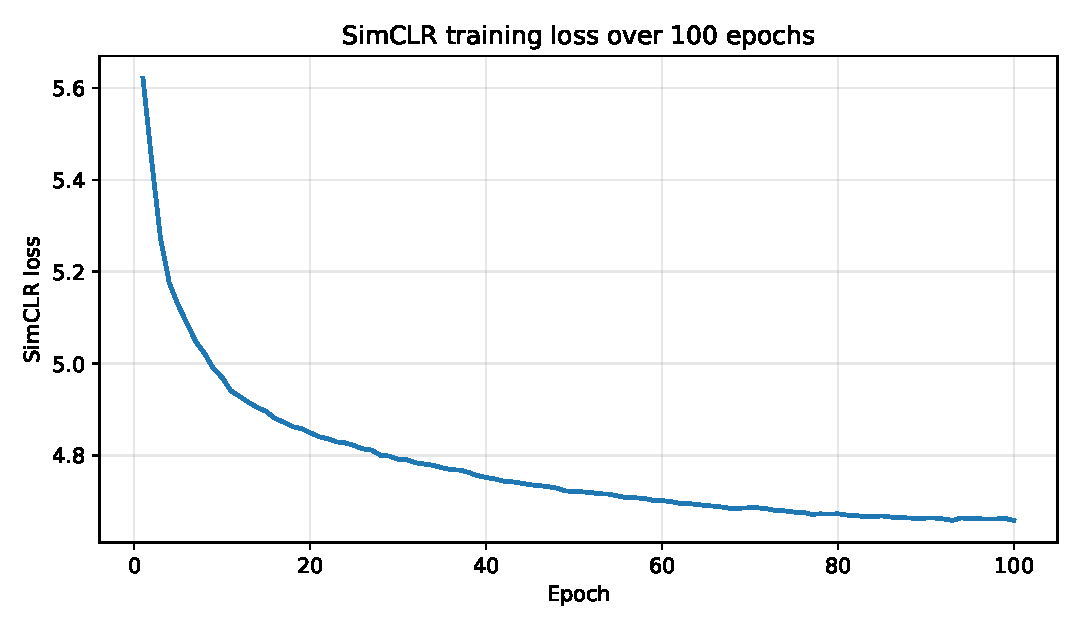
\includegraphics[width=0.78\textwidth]{final_training_loss.pdf}
\caption{SimCLR training loss over 100 epochs from the final run log.}
\label{fig:training-loss}
\end{figure}

The decrease is strongest during the first epochs. After roughly epoch 70, the loss changes more slowly and oscillates around a lower value. This does not prove that the representation is optimal, but it shows that the contrastive objective was optimized across the full scheduled run.

\begin{table}[H]
\centering
\caption{Selected SimCLR loss values from the final run.}
\begin{tabular}{rrrrrrrr}
\toprule
Epoch & 1 & 10 & 25 & 50 & 75 & 90 & 100\\
\midrule
Loss & 5.6214 & 4.9697 & 4.8217 & 4.7216 & 4.6768 & 4.6637 & 4.6586\\
\bottomrule
\end{tabular}
\end{table}

\subsection{Official CIFAR-10-C status}

The official CIFAR-10-C evaluation was not completed in the provided log. The attempted run failed before accuracy computation because \texttt{shot\_noise.npy} was not found in the expected directory. Table~\ref{tab:cifar10c-status} separates confirmed results from missing benchmark elements.

\begin{table}[H]
\centering
\caption{Status of the available evaluation evidence.}
\label{tab:cifar10c-status}
\begin{tabularx}{\textwidth}{>{\raggedright\arraybackslash}p{0.34\textwidth}>{\raggedright\arraybackslash}X}
\toprule
Item & Status\\
\midrule
Completed 100-epoch SSL run & Confirmed by terminal output.\\
Final linear evaluation accuracy & Confirmed: 67.05\%.\\
Available baseline and TTT accuracies & Confirmed by terminal output: 48.34\% and 55.78\%.\\
Official \texttt{shot\_noise.npy} run & Failed with \texttt{FileNotFoundError}.\\
Full TTT results CSV & Not provided in the available results.\\
Per-corruption table over 15 CIFAR-10-C corruptions & Not provided in the available results.\\
Mean accuracy over all CIFAR-10-C corruptions & Not provided in the available results.\\
\bottomrule
\end{tabularx}
\end{table}

% =================================================
\section{Analysis and Discussion}
% =================================================

The final available evaluation gives 48.34\% accuracy without adaptation and 55.78\% after ActMAD TTT. The gain is 7.44 percentage points. This result supports the idea that activation matching can help under the evaluated shift, but it is not enough to claim full robustness on CIFAR-10-C.

The baseline accuracy under the available shifted or corrupted evaluation is lower than the 67.05\% linear evaluation accuracy. This is consistent with the distribution-shift problem. The classifier works better on the clean evaluation setting than on the shifted test setting. The drop does not come from a new class set, because the CIFAR-10 classes remain the same. It comes from the change in image statistics seen by the backbone and classifier.

The ActMAD result recovers part of the lost performance. Matching target activation statistics to source activation statistics can move the adapted model toward the distribution on which the classifier was trained. In this run, that movement improved accuracy rather than damaging it. The improvement is large enough to be meaningful for the available evaluation: +7.44 percentage points is not just a rounding effect.

The result should still be interpreted carefully. First, the representation quality is moderate. A 67.05\% linear evaluation accuracy shows that SimCLR learned useful features, but the encoder is not a very strong CIFAR-10 classifier. If the representation were stronger, the baseline and TTT results could change. If the representation were weaker, adaptation could become unstable or meaningless.

Second, the result is not per-corruption. CIFAR-10-C is useful because it separates corruptions. Noise, blur, weather effects, and digital artifacts do not necessarily affect the model in the same way. A single available evaluation cannot show whether ActMAD helps on noise but fails on fog, or helps on compression but fails on contrast. A complete robustness claim would need the full 15-corruption table.

Third, the failed \texttt{shot\_noise.npy} attempt matters. It proves that at least one official CIFAR-10-C file was missing at the time of the run. The report therefore avoids saying that the final TTT numbers are official CIFAR-10-C benchmark results. They are reported as the final available TTT evaluation.

Fourth, test-time adaptation is not automatically safe. The model adapts without labels. A lower activation matching loss does not guarantee better classification. If the target batch is small, unbalanced, or too severely corrupted, the statistics can be misleading. The optimizer may make the activations look more source-like while losing class-discriminative information. This is why future experiments should keep negative results visible and not only report successful cases.

The main positive point is that the implemented pipeline is coherent. The SSL stage produces a usable backbone, the linear classifier gives a representation-quality check, source statistics are saved, and TTT loads the saved files and performs adaptation. The main weak point is experimental coverage. The available result is a useful final run for the TER report, but a stronger scientific conclusion would require the official CIFAR-10-C files and a full per-corruption evaluation.

% =================================================
\section{Limitations}
% =================================================

The first limitation is the missing official CIFAR-10-C file. The provided log shows a \texttt{FileNotFoundError} for:
\begin{lstlisting}
data/raw/cifar10c/CIFAR-10-C/shot_noise.npy
\end{lstlisting}
Because of that, the official CIFAR-10-C evaluation was not completed in the available log.

The second limitation is the absence of a full result CSV. No final \texttt{results/test\_time\_training/results.csv} was provided. The final TTT numbers in this report come from terminal output. This is acceptable for reporting the available run, but a CSV is better for reproducibility because it fixes the exact corruption, severity, batch size, adaptation steps, and learning rate for each row.

The third limitation is the missing per-corruption table. CIFAR-10-C contains several corruption families. A single available TTT number cannot show whether the method is robust across noise, blur, weather, and digital corruptions. No comparison over all 15 CIFAR-10-C corruptions is available in the final results.

The fourth limitation is representation quality. The final linear evaluation accuracy is 67.05\%. This is a useful result for a self-supervised Master 1 implementation, but it is not a strong final CIFAR-10 classifier. A stronger backbone might give a different baseline and a different adaptation behavior.

The fifth limitation is hyperparameter search. The report uses the available ActMAD setting with ten adaptation steps and learning rate \(10^{-4}\). No systematic comparison of step counts, batch sizes, learning rates, or adaptation parameter subsets was provided. The reported improvement should therefore be read as a result for one available setting, not as an optimized TTT configuration.

The sixth limitation is adaptation instability. ActMAD aligns activation statistics, not labels. A lower activation matching loss does not guarantee better classification. This is a known difficulty in test-time adaptation and should be considered when interpreting positive and negative results.

The method should be validated again after placing the official CIFAR-10-C \texttt{.npy} files in:
\begin{lstlisting}
data/raw/cifar10c/CIFAR-10-C/
\end{lstlisting}
Then the full script can produce per-corruption results and mean accuracy values.

% =================================================
\section{Reproducibility}
% =================================================

The main commands from the repository root are:
\begin{lstlisting}
python run.py --task self_supervised --config configs/self_supervised.yaml
python run.py --task test_time_training --config configs/test_time_training.yaml
python run.py --task ssl --config configs/self_supervised.yaml
python run.py --task ttt --config configs/test_time_training.yaml
python scripts/eval_corruption.py
\end{lstlisting}

The expected order is to run self-supervised training first. This creates the backbone, classifier, and source activation statistics under \texttt{results/self\_supervised/}. The TTT stage then loads these files. The confirmed saved files are:
\begin{lstlisting}
results/self_supervised/simclr_backbone.pt
results/self_supervised/classifier.pt
results/self_supervised/source_stats.pt
\end{lstlisting}

TTT numerical results are expected in:
\begin{lstlisting}
results/test_time_training/results.csv
\end{lstlisting}
when the local code writes the CSV. If this file is missing, the terminal output remains the source for the available baseline and adapted accuracies. The final available terminal output reports 48.34\% baseline accuracy, 55.78\% ActMAD TTT accuracy, and +7.44 percentage points of improvement.

For official CIFAR-10-C, the \texttt{.npy} files must exist under:
\begin{lstlisting}
data/raw/cifar10c/CIFAR-10-C/
\end{lstlisting}
The missing \texttt{shot\_noise.npy} file must be corrected before reporting official CIFAR-10-C results. The labels file \texttt{labels.npy} must also be present.

The terminal warnings observed during the provided run are not central to the scientific method. The MPS warning says that \texttt{pin\_memory=True} is not supported on MPS, so pinned memory is not used. This can be cleaned by setting \texttt{pin\_memory=False} when the device is MPS. The NumPy deprecation warning comes from dataset loading and does not change the reported accuracy values, but a stable dependency combination is safer for repeated experiments.

% =================================================
\section{Final Remarks and Future Work}
% =================================================

The project implements a complete pipeline for self-supervised test-time adaptation on image classification. SimCLR trains a ResNet18 backbone on CIFAR-10. A linear classifier evaluates the learned representation. Source activation statistics are computed on clean data. At test time, ActMAD-style adaptation updates normalization parameters on unlabeled corrupted batches before classification.

The final available results are positive but limited. The self-supervised run completed 100 epochs and reached 67.05\% linear evaluation accuracy. The available TTT evaluation improved accuracy from 48.34\% to 55.78\%, a gain of 7.44 percentage points. This supports the usefulness of activation matching in the evaluated setting.

The result is not a complete robustness benchmark. The official CIFAR-10-C run failed when \texttt{shot\_noise.npy} was missing, and no per-corruption CSV was provided. A stronger final experiment would use the official CIFAR-10-C files, evaluate all 15 corruptions, report mean accuracy, and compare several adaptation settings.

The next practical steps are clear: install the official CIFAR-10-C \texttt{.npy} files, run \texttt{scripts/eval\_corruption.py}, save the resulting CSV, and compare ActMAD across corruptions and severity levels. It would also be useful to test several adaptation step counts, several batch sizes, and at least one other test-time adaptation method. Safer adaptation criteria should also be studied, because an unsupervised adaptation loss can improve activation matching while hurting classification.

% =================================================
\section{References}
% =================================================

\begin{thebibliography}{9}

\bibitem[Chen et~al.(2020)]{chen2020simclr}
T. Chen, S. Kornblith, M. Norouzi, and G. Hinton.
\newblock A Simple Framework for Contrastive Learning of Visual Representations.
\newblock In \emph{Proceedings of the 37th International Conference on Machine Learning}, 2020.

\bibitem[Sun et~al.(2020)]{sun2020ttt}
Y. Sun, X. Wang, Z. Liu, J. Miller, A. A. Efros, and M. Hardt.
\newblock Test-Time Training with Self-Supervision for Generalization under Distribution Shifts.
\newblock In \emph{Proceedings of the 37th International Conference on Machine Learning}, 2020.

\bibitem[Liu et~al.(2021)]{liu2021tttpp}
Y. Liu, P. Kothari, B. G. van Delft, B. Bellot-Gurlet, T. Mordan, and A. Alahi.
\newblock TTT++: When Does Self-Supervised Test-Time Training Fail or Thrive?
\newblock In \emph{Advances in Neural Information Processing Systems}, 2021.

\bibitem[Hendrycks and Dietterich(2019)]{hendrycks2019robustness}
D. Hendrycks and T. Dietterich.
\newblock Benchmarking Neural Network Robustness to Common Corruptions and Perturbations.
\newblock In \emph{International Conference on Learning Representations}, 2019.

\bibitem[Mirza et~al.(2023)]{mirza2023actmad}
M. J. Mirza, P. Jan\'{e} Soneira, W. Lin, M. Kozinski, H. Possegger, and H. Bischof.
\newblock ActMAD: Activation Matching to Align Distributions for Test-Time-Training.
\newblock In \emph{Proceedings of the IEEE/CVF Conference on Computer Vision and Pattern Recognition}, 2023.

\bibitem[Krizhevsky(2009)]{krizhevsky2009cifar}
A. Krizhevsky.
\newblock Learning Multiple Layers of Features from Tiny Images.
\newblock Technical report, University of Toronto, 2009.

\bibitem[He et~al.(2016)]{he2016resnet}
K. He, X. Zhang, S. Ren, and J. Sun.
\newblock Deep Residual Learning for Image Recognition.
\newblock In \emph{Proceedings of the IEEE Conference on Computer Vision and Pattern Recognition}, 2016.

\end{thebibliography}

\end{document}
